\chapter{Modulo 5}\label{cap : Mod5}

\section{DEEP INELASTIC SCATTERING \textcolor{blue}{*}}

In questo capitolo si analizzerà uno degli esperimenti che ha prodotto forti evidenze riguardo il modello a quark. Per \textit{deep inelastic scattering} si intende lo scattering tra elettrone e protone che avviene con un impulso trasferito elevato (sopra $1 Gev$). In tale regime si osserva un basso rate di collisioni elastiche, la maggior parte degli eventi produce un gran numero di adroni, si può quindi investigare la struttura interna del protone. Il deep inelastic scattering è analizzato considerando l'elettrone incidente interagisca con un quark libero del protone. Tale approssimazione può sembrare sorprendente, trascura infatti il legame forte tra i quark del protone. Giustificheremo tale fenomeno introducendo il concetto di \textbf{Asymptotic freedom} 

\subsection{SLAC-MIT experiment}

L'esperimento è stato condotto nel 1968 al Stanford Linear Accelerator (SLAC). Fasci di elettroni di energia $7-17 Gev$ venivano accelerati su bersagli di idrogeno (7 cm target). Il punto centrale dell'esperimento era la misura delle variabili cinematiche dell'elettrone uscente con precisione, determinando l'impulso trasferito al protone. L'impulso dell'elettrone veniva misurato tramite spettrometri magnetici, con la possibilità di ruotarli intorno al bersaglio per esplorare diversi angoli di scattering per gli elettroni uscenti. La configurazione dei detector permetteva la misura fino a $7.4 Gev$ di momento trasferito al protone.

\begin{figure}[hbtp]
\centering
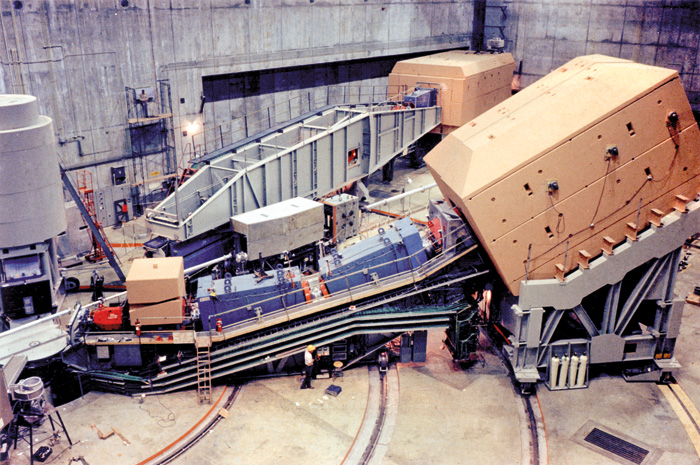
\includegraphics[scale=0.5]{CCsla3_09_12.jpg}
\caption{Struttura dell'esperimento, a destra si notato gli spettrometri con i calorimetri per discernere i pioni dagli elettroni. Il bersaglio di idrogeno è situato a sinistra, sotto il cilindro. Gli spettrometri potevano essere ruotati sui binari presenti in foto }
\end{figure}

Lo scopo dell'esperimento era quello di analizzare i costituenti interni del protone, ponendo attenzione alla misura dell'elettrone scatterato ed ignorando gli adroni nello stato finale. Il diagramma che descrive il processo 
\begin{center}

\feynmandiagram [horizontal=a to b] {
i1 [particle=\(e^{-}\)] -- [fermion] a -- [fermion] i2 [particle=\(e^{-}\)],
a -- [photon] b [blob],
f1 [particle=\(W\)]-- [anti fermion] b -- [anti fermion] f2 [particle=\(p\)] ,
};
\end{center}

Dove con $W$ indichiamo lo stato adronico finale. La corrente associata al vertice fotone-protone è un oggetto abbastanza complesso, bisogna fare alcune ipotesi, che portano sostanzialmente a formulare il modello a partoni, per poter scrivere l'ampiezza. Prima di procedere si fa un veloce richiamo al più semplice scattering elastico protone elettrone, studiato negli anni 50 da Robert Hofstadter a Stanford.

\paragraph{Sezione d'urto Rutherford}

Riportiamo velocemente una derivazione della sezione d'urto Rutherford utilizzando però gli opportuni limiti in teoria di campo. Nello scattering si ignora il rinculo del protone e si considera l'elettrone non relativistico. Gli spinori che descrivono il processo si scrivono :

\begin{equation}
\sqrt{E + m}\cdot
\left (\begin{array}{c}
• c \\ 
• s e^{i\phi} \\ 
• c K\\ 
• s K e^{i\phi}
\end{array} \right )
\end{equation}